\begin{figure}
	\centering
	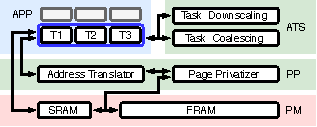
\includegraphics[width=\columnwidth]{figures/system-overview.pdf}
	\caption{\sys top-level view. ATS: adaptive task scheduler, VMM: virtual memory manager, PM: physical memory.}
	\label{fig:system_overview}
\end{figure}

\sys is a new programming and execution model for intermittent operation on energy-harvesting devices. It addresses the challenges given in Section~\ref{sec:background} making task-based intermittent applications {\em programmable}, {\em efficient} and {\em portable}, introducing a new programming model and runtime software system that supports adaptive task-based execution. Fig.~\ref{fig:system_overview} shows an overview of \sys.

\paragraph{Programming and Execution Model.}
To use \sys, a programmer must (i) convert a plain C code into tasks by encapsulating the code in a top-level set of functions, (ii) sequence the control-flow between these tasks, and (iii) annotate memory accesses that manipulate task-shared data. Then, they compile and link the code against \sys's runtime, producing a \sys-enabled binary. The runtime relies on \sys's novel {\em adaptive task scheduler} to adapt its execution with the energy conditions. Facilitating efficient task adaptation requires dynamic memory protection which \sys's \emph{virtual memory manager} handles through a process we call \emph{dynamic page privatization}. 

\paragraph{Adaptive Task Scheduler.}
\sys's adaptive task scheduler (ATS) makes \emph{energy-aware} scheduling decisions to group tasks together or split a task. By coalescing tasks \sys \emph{amortizes commit and transition costs}, and by splitting a task, after it repeatedly failed to complete, it \emph{avoids the task non-termination problem}. The scheduler uses its recent execution history---i.e., it is hardware independent---as a metric to estimate energy availability and eventually to decide on the coalesced task size. Section~\ref{sec:task_adaptation} describes ATS.

\paragraph{Virtual Memory Manager.}
\sys can coalesce tasks thanks to its virtual memory manager (VMM). VMM privatizes memory pages demanded by a coalesced task and limits application accesses only to the fast volatile memory. VMM keeps all page modifications in non-volatile memory on a coalesced task transition. Section~\ref{sec:memory_virtulaization} outlines VMM.
